%----------------------------------------------------------------------------------------
%	PACKAGES AND THEMES
%----------------------------------------------------------------------------------------
\documentclass[aspectratio=169,xcolor=dvipsnames,]{beamer}
\usetheme{Darmstadt}
\usecolortheme{seahorse}

\usepackage[hangul]{kotex}

\usepackage{hyperref}
\usepackage{amsfonts, amssymb}
\usepackage{graphicx} % Allows including images
\usepackage{booktabs, multicol, multirow} % Allows the use of \toprule, \midrule and \bottomrule in tables
\setbeamercovered{transparent}

\newcommand{\R}{\mathbb{R}}
\newcommand{\y}{\mathbf{y}}

%----------------------------------------------------------------------------------------
%	TITLE PAGE
%----------------------------------------------------------------------------------------

\title[불평등지수]{불평등지수} % The short title appears at the bottom of every slide, the full title is only on the title page
\subtitle{경제정의와 불평등}

\author[오성재]{오성재}

\institute[HNU] % Your institution as it will appear on the bottom of every slide, may be shorthand to save space
{
    한남대학교 \\
    탈메이지 교양학부 \\
}
\date{\today} % Date, can be changed to a custom date


%----------------------------------------------------------------------------------------
%	PRESENTATION SLIDES
%----------------------------------------------------------------------------------------

\begin{document}

\begin{frame}
    % Print the title page as the first slide
    \titlepage
\end{frame}

\begin{frame}{목차}
    \tableofcontents
\end{frame}
%------------------------------------------------

\begin{frame}[<+->]
\frametitle{학습목표}
    \begin{itemize}
        \item 불평등지수가 갖춰야 할 바람직한 특성 이해.
        \item 개별 불평등 지수들의 특성 이해.
    \end{itemize}
\end{frame}
%------------------------------------------------

%------------------------------------------------
\section{불평등 지수의 특성}
%------------------------------------------------

\begin{frame}[<+->]
\frametitle{개념들}
    \begin{itemize}
        \item 사회 : $(N, \mathbf{y})$.
        \begin{itemize}
            \item 사람 : $N = \{1,2, \ldots , n \}$.
            \item 소득분포 : $\mathbf{y} = \{y_1,y_2, \ldots , y_n \} \in \R ^n$.
            \item 소득분포의 집합: $\Omega = \{ \y | \text{가능한 모든 소득 분포 } \y \text{ 의 집합}\}$.
        \end{itemize}
        \item 불평등 지수 : $I : \Omega \rightarrow \R$
        \begin{itemize}
            \item 가능한 모든 소득분포를 실수에 대입하는 함수.
        \end{itemize}
    \end{itemize}
\end{frame}
%------------------------------------------------

\begin{frame}[<+->]
\frametitle{불평등지수의 특성I}
    \begin{itemize}
        \item 평준화 : 소득분포가 완전평등이면 불평등 지수는 0 값을 가지고 아니라면 양수 값을 가져야 한다.
        \item 대칭성(익명성) : 불평등 지수는 소득분포에만 근거해야 한다.
        \begin{itemize}
            \item 만약 $\y '$라는 소득분포가 같은 $N$명의 소득분포 $\y$에서 단순히 사람의 이름만을 바꾼 분포라면 불평등 지수는 같은 값을 가져야 한다. 즉, $I(\y) = I=(\y ')$ 이다.
        \end{itemize}
        \item 인구복사 : 동일한 소득분포를 가진 인구를 단순히 복제한 경우라면 불평등 지수는 동일해야 한다.
    \end{itemize}
\end{frame}
%------------------------------------------------

\begin{frame}[<+->]
\frametitle{불평등지수의 특성II}
    \begin{itemize}
        \item 피구-달튼(Pigou-Dalton) 이전 원칙 :  
        \begin{itemize}
            \item 총 소득에 변화가 없이 부자에서 빈자에게 소득이 이전되는 것을 달튼 이전이라고 하자. 
            \item 달튼이전이 일어나면 불평등 지수는 감소해야 한다.
        \end{itemize}
    \begin{block}{Dalton(1920), Pigou(1912)}
    임의의 소득분포 $\y = \{y_1 ,y_2 , \ldots , \ldots ,y_n \}$ 에 대하여 $\y ' = \{y_1 ,y_2 , \ldots , y_i + \delta , y_j - \delta , \ldots ,y_n \}$ 는 임의의 두 사람 $i$와 $j$간에 달튼 이전이 일어난 소득분포라고 하자($y_i \leq y_j$). 그렇다면 $I(\y) < I(\y ')$ 이어야 한다.
    \end{block}
    \item 고려사항
    \begin{itemize}
        \item 크기 : 이전된 소득규모에 대하여 불평등 지수가 얼마냐 변하는가에 무관하다.
        \item 분포상의 위치 : 부자에서 덜 부자 vs. 빈자에서 더 빈자.
    \end{itemize}
    \end{itemize}
\end{frame}
%------------------------------------------------

\begin{frame}[<+->]
\frametitle{불평등지수의 특성III}
    \begin{itemize}
        \item 규모의 독립성 : 모두가 같은 비율로 소득이 변한다면, 불평등 지수는 변화가 없어야 한다.
        \begin{itemize}
            \item 임의의 양수 $\lambda > 0$와 모든 소득분포 $\y$에 대하여 $I(\lambda \y) = I(\y)$.
            \item 불평등 지수는 {\bf 상대적 지수} 이다.
        \end{itemize}
        \item 가산적 분해성 : 인구를 임의의 집단으로 나눴을때 불평등 지수는 집단내 불평등과 집단간 불평등의 합으로 나타낼 수 있어야 한다.
        \begin{itemize}
            \item $g$를 집단의 표시, $\omega _g$를 집단의 비율, $\y ^g$를 $g$ 집단에 속한 사람들만의 소득분포라고 할 때, 
        \end{itemize}
        $$ I(\y) = \sum _g \omega _g I(\y ^g) + I(\cdot).$$
    \end{itemize}
\end{frame}
%------------------------------------------------
\section{불평등과 퍼짐}
\begin{frame}[<+->]
    \begin{itemize}
        \item 불평등과 퍼짐은 밀접한 관련이 있지만 구분해야 하는 개념이다.
    \begin{exampleblock}{예시}
        $\y _1 = ( 10, 20, 30, 40, 100)$ $\y _2 = ( 24, 24, 24, 24, 104)$ 은 합이 200으로 동일한 두 분포이다. 
    \end{exampleblock}
    \item 3명에게는 $\y _2$에서 소득이 더 높다.
    \item 20이 절대수준이라면 $\y _2$가 더 낫다.
    \end{itemize}
\end{frame}
%------------------------------------------------

\begin{frame}[<+->]
\frametitle{분산($\sigma ^2$)}
    \begin{itemize}
        \item 대표적인 퍼짐의 척도 :  
        $$ \sigma ^2  = \frac{1}{n} \sum _{i=1} ^n (y_i - \mu)^2 \text{또는}$$
        $$ \sigma ^2  = \frac{1}{n} \sum _{i=1} ^n (y_i^2 - \mu^2) \text{또는}$$
        \item 규모의 독립성은 만족하지 못한다.
        \item $\sigma ^2 (\y _1)= 1000$, $\sigma ^2 (\y _2)= 1024= 1024$.
    \end{itemize}
\end{frame}
%------------------------------------------------

\begin{frame}[<+->]
\frametitle{분산계수(coefficient of variation(CV)}
    \begin{itemize}
        \item 소득분포 $\y$의 표준편차를 평균값으로 나눈 값:
        $$ CV = \frac{\sigma}{\mu}.$$ 
        \item 가산적 분해성은 상실하지만 규모의 독립성은 만족.
    \end{itemize}
\end{frame}
%------------------------------------------------
\section{불평등 지수} 
\begin{frame}[<+->]
\frametitle{로렌츠 곡선(Lorenz curve)I}
    \begin{itemize}
        \item 소득분포 $\mathbf{y} = \{y_1,y_2, \ldots , y_n \}$가 소득의 크기 순서대로 정렬되어 있다고 가정($y_1 \leq y_2 \leq \ldots \leq y_n$).
        \item 로렌츠 곡선은 다음의 두 좌표 $(p_i , L(p_i))$의 조합이다.
        \begin{itemize}
            \item $p_i$ : $y_i$ 보다 소득이 적거나 같은 사람의 비중.
            \item $L(p_i)$ : 총 소득에서 $y_i$보다 소득이 적거나 같은 사람의 소득이 차지하는 비중: 
                $$L(p_i) = \frac{\sum ^i _{j=1} y _j}{n \mu}.$$
            \item $L(0) = 0$ , $L(1) = 1$.
        \end{itemize}
        
    \end{itemize}
\end{frame}
%------------------------------------------------

\begin{frame}
\frametitle{로렌츠 곡선(Lorenz curve)II}
    \begin{columns}
        \begin{column}{.5\textwidth}<1->
            \begin{figure}
                \centering
                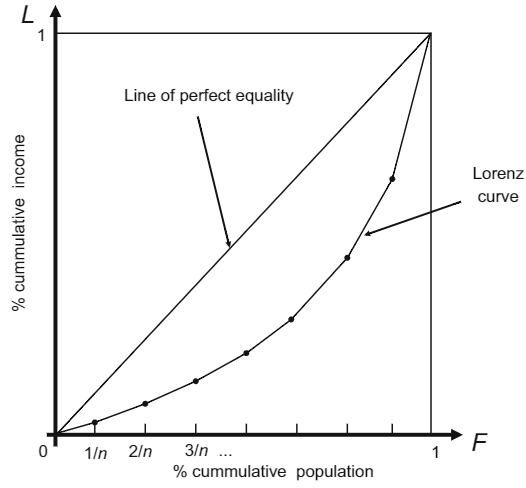
\includegraphics[width=.78\textwidth]{pic/lorenz.png}
                \caption{로렌츠 곡선}
            \end{figure}
        \end{column}
        \begin{column}{.5\textwidth}<2>
            \begin{figure}
                \centering
                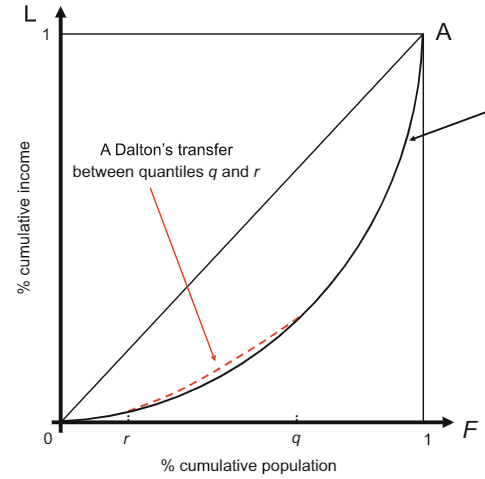
\includegraphics[width=.78\textwidth]{pic/lorenzt.png}
                \caption{로렌츠 곡선으로 본 이전}
            \end{figure}
        \end{column}
    \end{columns}
\end{frame}

\begin{frame}
\frametitle{로렌츠 곡선(Lorenz curve)III}
    \begin{columns}
        \begin{column}{.5\textwidth}<1->
            \begin{figure}
                \centering
                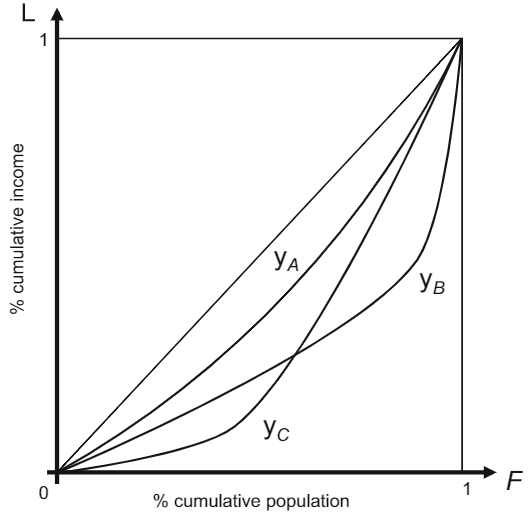
\includegraphics[width=.78\textwidth]{pic/lorenzd.png}
                \caption{로렌츠 지배}
            \end{figure}
        \end{column}
        \begin{column}{.5\textwidth}<2>
            \begin{itemize}
                \item {\bf 로렌츠 지배} : 하나의 로렌츠 곡선이 항상 다른 로렌츠 곡선의 위에 있을 경우.
                \item 서로다른 로렌츠 곡선이 교차하는 경우에 대한 판별이 불가능.
                \item 순서적 개념이고, 정도를 측정할 수 없음.
            \end{itemize}
        \end{column}
    \end{columns}
\end{frame}
%------------------------------------------------

\begin{frame}[<+->]
\frametitle{지니 계수(Gini index)}
    \begin{columns}
        \begin{column}{.5\textwidth}<1->
            \begin{figure}
                \centering
                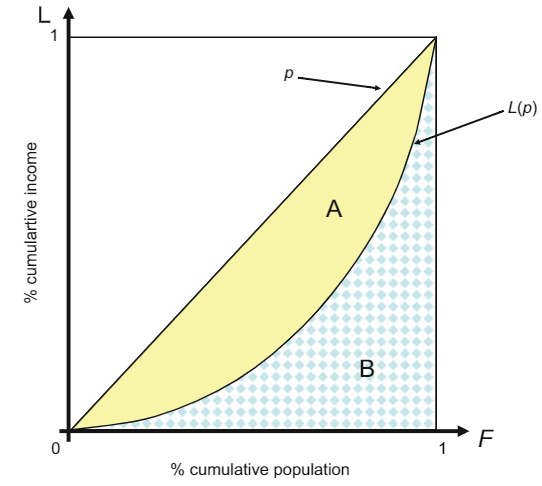
\includegraphics[width=.78\textwidth]{pic/gini.png}
                \caption{지니계수}
            \end{figure}
        \end{column}
        \begin{column}{.5\textwidth}<2>
            \begin{itemize}
                \item 지니계수(G) :
                $$ G = \frac{A}{A+B}$$   
                \item 전체인구의 평균소득 격차를 $\Delta$ 라고 하자 : 
                $$ \Delta = \frac{1}{n^2}\sum _i \sum _j | y_i - y_j |, \quad G = \frac{\Delta}{2 \mu}.$$
                \item 가산적 분해성은 없음.
            \end{itemize}
        \end{column}
    \end{columns}
\end{frame}
%------------------------------------------------

\begin{frame}[<+->]
\frametitle{분위 척도}
    \begin{itemize}
        \item 5분위배율 :
        $$Q= \frac{ \text{상위 20\% 소득점유 비율} }{ \text{하위 20\% 소득점유 비율} }.$$
        \item 이외에도 10-90비율, 20-20비율, 중위-평균 비율 등이 존재.
            \begin{itemize}
                \item 계산이 용이하고 직관적임.
                \item 그러나 피구-달튼 원칙을 위배.
                \item (국가간, 시점간, 집단간)불평등에 대한 비교에서는 부적절함.
            \end{itemize}
    \end{itemize}
\end{frame}
%------------------------------------------------

\begin{frame}[<+->]
\frametitle{팔마비율(Palma ratio)}
    \begin{itemize}
        \item 팔마비율(Palma ratio) :
        $$Q= \frac{ \text{상위 10\% 소득점유 비율} }{ \text{하위 40\% 소득점유 비율} }.$$
            \begin{itemize}
                \item 소득 10분위에서 5-9분위의 40\% 인구는 전체소득의 약 50\%를 안정적으로 점유.
                \item 소득분배의 변화에 실질적인 영향을 받는 나머지 60\% 인구를 포착.
                \item 지니계수가 중간층에 너무 민감하다는 단점을 보완.
            \end{itemize}
    \end{itemize}
\end{frame}
%------------------------------------------------

\begin{frame}[<+->]
\frametitle{균등분배 대등소득(Equally distributed equivalent income;EDIE)}
    \begin{itemize}
        \item 앞서의 불평등 척도는 자료를 통한 분배의 형태만을 고려.
        \item 불평등 척도에 가치판단을 도입이 요구됨.
        \item EDEI는 사회후생수준의 판단에 따라 상이하다.
        \begin{itemize}
            \item 주어진 $\mathbf{y} = \{y_1,y_2, \ldots , y_n \}$에 대하여 소득의 평균은 $\mu$이고 이 소득분포가 달성하는 사회후생의 수준을 $SW(\mathbf{y})$라고 하자.
            \item 그리고 $n$명의 사람이 동일하게 $y$라는 소득을 얻는 분포를 $ y \cdot I_n$라고 하자.
            \item 균등분배 대등소득 $y_e$는 $SW(\y) = SW(y_e \cdot I_n)$을 만족하는 소득이다.  
        \end{itemize}
    \end{itemize}
\end{frame}
%------------------------------------------------

\begin{frame}[<+->]
\frametitle{균등분배 대등소득 계산}
    \begin{exampleblock}{5인 사회에서 EDID 계산}
        \begin{itemize}
            \item 5인의 소득이 $\mathbf{y} = \{12, 25, 3, 23, 7\}$로 주어져 있다.
            \item 공리주의 : $SW = 12+25+3+23+7 = 70$. $y_e = \frac{70}{5}=14$.
            \item 하이에크 : $SW = 12\times25\times3\times23\times7 = 144900$. $y_e = \sqrt[5]{144990}=10.77$.
            \item 롤즈 : $SW = min(12,25,3,23,7) = 3$. $y_e = 3$
        \end{itemize}
    \end{exampleblock}
\end{frame}
%------------------------------------------------

\begin{frame}[<+->]
\frametitle{앳킨슨 지수(Atkinson index)}
    \begin{columns}
        \begin{column}{.5\textwidth}
            \begin{figure}
                \centering
                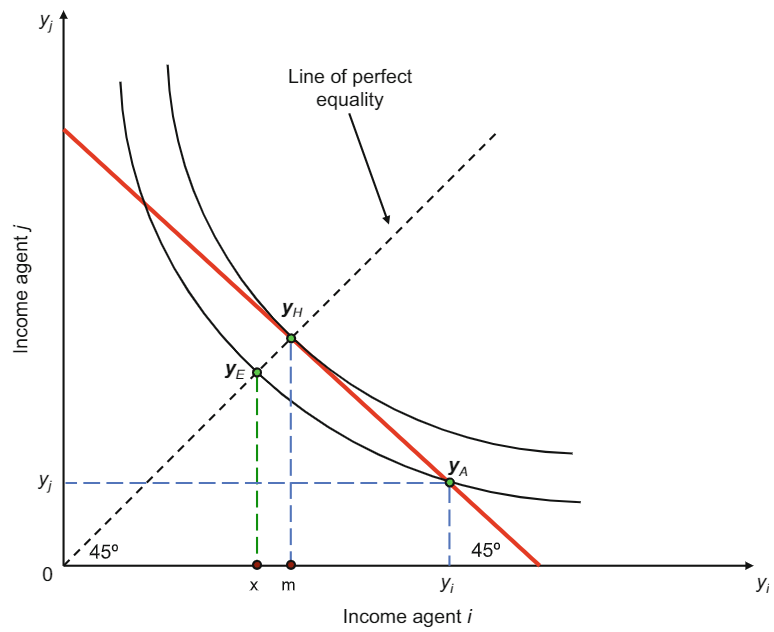
\includegraphics[width=.78\textwidth]{pic/eqincome.png}
                \caption{균등분배 대등소득}
            \end{figure}
        \end{column}
        \begin{column}{.5\textwidth}
            \begin{itemize}
                \item 주어진 $\mathbf{y} = \{y_1,y_2, \ldots , y_n \}$에 대하여 소득의 평균은 $\mu$이고 이 소득분포가 달성하는 사회후생의 수준이 $SW(\mathbf{y})$일때 EDEI는 $y_e$라고 하자.
                \item 앳킨슨 지수 A는 다음과 같다:
                $$A = 1- \frac{y_e}{\mu}.$$
            \end{itemize}
        \end{column}
    \end{columns}
\end{frame}
%------------------------------------------------

\end{document}